\documentclass[a4j,8pt,twocolumn]{extarticle}

% ---------------

\usepackage{winf-paper}
\usepackage{amsmath}
\usepackage{amssymb}
\usepackage{ascmac}
\usepackage{latexsym}
\usepackage{ulem}
\usepackage[dvipdfmx]{graphicx}

% ---------------

%% 和文題目
\title{行動パターンを用いた置き忘れ防止システムの開発に関する研究}

%% 和文著者
\author{大橋 世弥}

%% 和文所属
\affiliation{愛知工業大学 情報科学部 情報科学科}





% ===== 所属が複数の場合 =====
%\author{情報 太郎\DAG{1} \qquad 情報 花子\DAG{1} \qquad 情報 次郎\DAG{2}}
%\affiliation{\DAG{1}情報大学情報学部 \qquad \DAG{2}情報大学大学院情報学研究科}
%\eauthor{Taro Info\DAG{1} \qquad Hanako Info\DAG{1} \qquad Jiro Info\DAG{2}}
%\eaffiliation{%
%	\DAG{1} Faculty of Information, Information University\\
%	\DAG{2} Graduate School of Information, Information University
%}

\begin{document}
	
\maketitle
\thispagestyle{empty}	% 1ページ目のページ番号を表示しない
% ------------------------------------------------------------

\section{はじめに}
日常の中では特定の物を一緒に持ち歩く習慣がある。
例えば学校に行くときはスマホと財布と通学カバンなどを持って外出したり,
自分の部屋からリビングに移動するときはスマホだけ持って移動したり,
ある時間には充電コードが必要なので研究室から教室へ充電コードを持って行ったりするかもしれない.

そのような物がある時間に特定の場所から特定の場所へ移動する状態を「時空間的に共起関係にある」と呼び,
本研究ではその共起関係の中から「外出の際の持ち物」について着目し,物の共起関係を用いて置き忘れを防止するためのシステムを開発していく.



% ------------------------------------------------------------
\section{関連研究}

\subsection{置き忘れ防止に関する研究}
置き忘れを防止するための研究の例として,人間行動を手がかりとしてそれが置き忘れなのか,物を置いて離席しただけなのかを判別する田中らの研究や,
加速度センサを用いてiPhoneの機能を組み合わせることで置き忘れたものとの距離や位置を特待する青田らの研究,
加速度センサとRFIDタグを用い電波強度と歩行推定を組み合わせて置き忘れを検知する北園らの研究がある.
また,MAMORIOやTileなどの置き忘れ防止グッズなども普及している.

これらの研究や物は実際に人や物の動きに着目し,事前に決めた置き忘れの基準を満たす場合にユーザに通知するシステムである.
また置き忘れをした後に通知する場合,状況によっては取り返しのつかない場合がある.
本システムではこうなった場合は置き忘れであると事前に決めず,外出の特徴を蓄積させていくことで自動的に置き忘れの状況を定義する.



\subsection{持ち物推定に関する研究}
持ち物推定をするための研究の例として,場所ごとに持ち物の情報を蓄積し分析する山岡らの研究や,
各持ち物の重さを事前に登録し外出時の持ち物を総重量から推定する浜野らの研究,
カメラ映像を用いて荷造りの際に持ち物を分析し後で必要だったかを判定する森田らの研究がある.

これらの研究は事前に状況を設定したり,ユーザ自身が評価したりする手間がかかり,
同じ場所に行くが,時間ごとに違う持ち物が必要な場合に対応していない.
そこで本研究では時間的,空間的に物同士の共起関係に着目する.


\subsection{探し物に関する研究}
置き忘れをした場合に忘れた物を探すための研究の例として,
超音波位置計測器とRFIDを用いて探し物の場所を推定し,照射して探す範囲を限定できる中田らの研究や,
探したい物と部屋の画像を比較して指定された物を探す佐藤らの研究,
最後にユーザの目の前で把持した時点の映像をユーザ自身が検索できるウェアラブルインタフェースを提案した上岡らの研究がある,

これらの研究は物を忘れた場合に部屋の情報を認識し忘れ物の場所を特定する,という手法が主である.
本研究では現在の情報をもとに場所を推定するのではなく,直前の外出の持ち物から何の近くにありそうか
を推定することによって忘れ物を探す支援をする.


% ------------------------------------------------------------
\section{置き忘れ防止システム「これ忘れていませんか」}

置き忘れ防止システム「これ忘れていませんか」は外出時間と持ち物から物の共起関係を探し,
持ち物予測及び置き忘れをユーザに知らせるシステムである.
そのため本システムは以下の図1で示すシステム構成図のように,物の移動を推定する,物の共起関係を探す,データを分析する,ユーザに知らせる,の大きく4つの手順から構成される.
\begin{figure}[tbh]
    \centering
    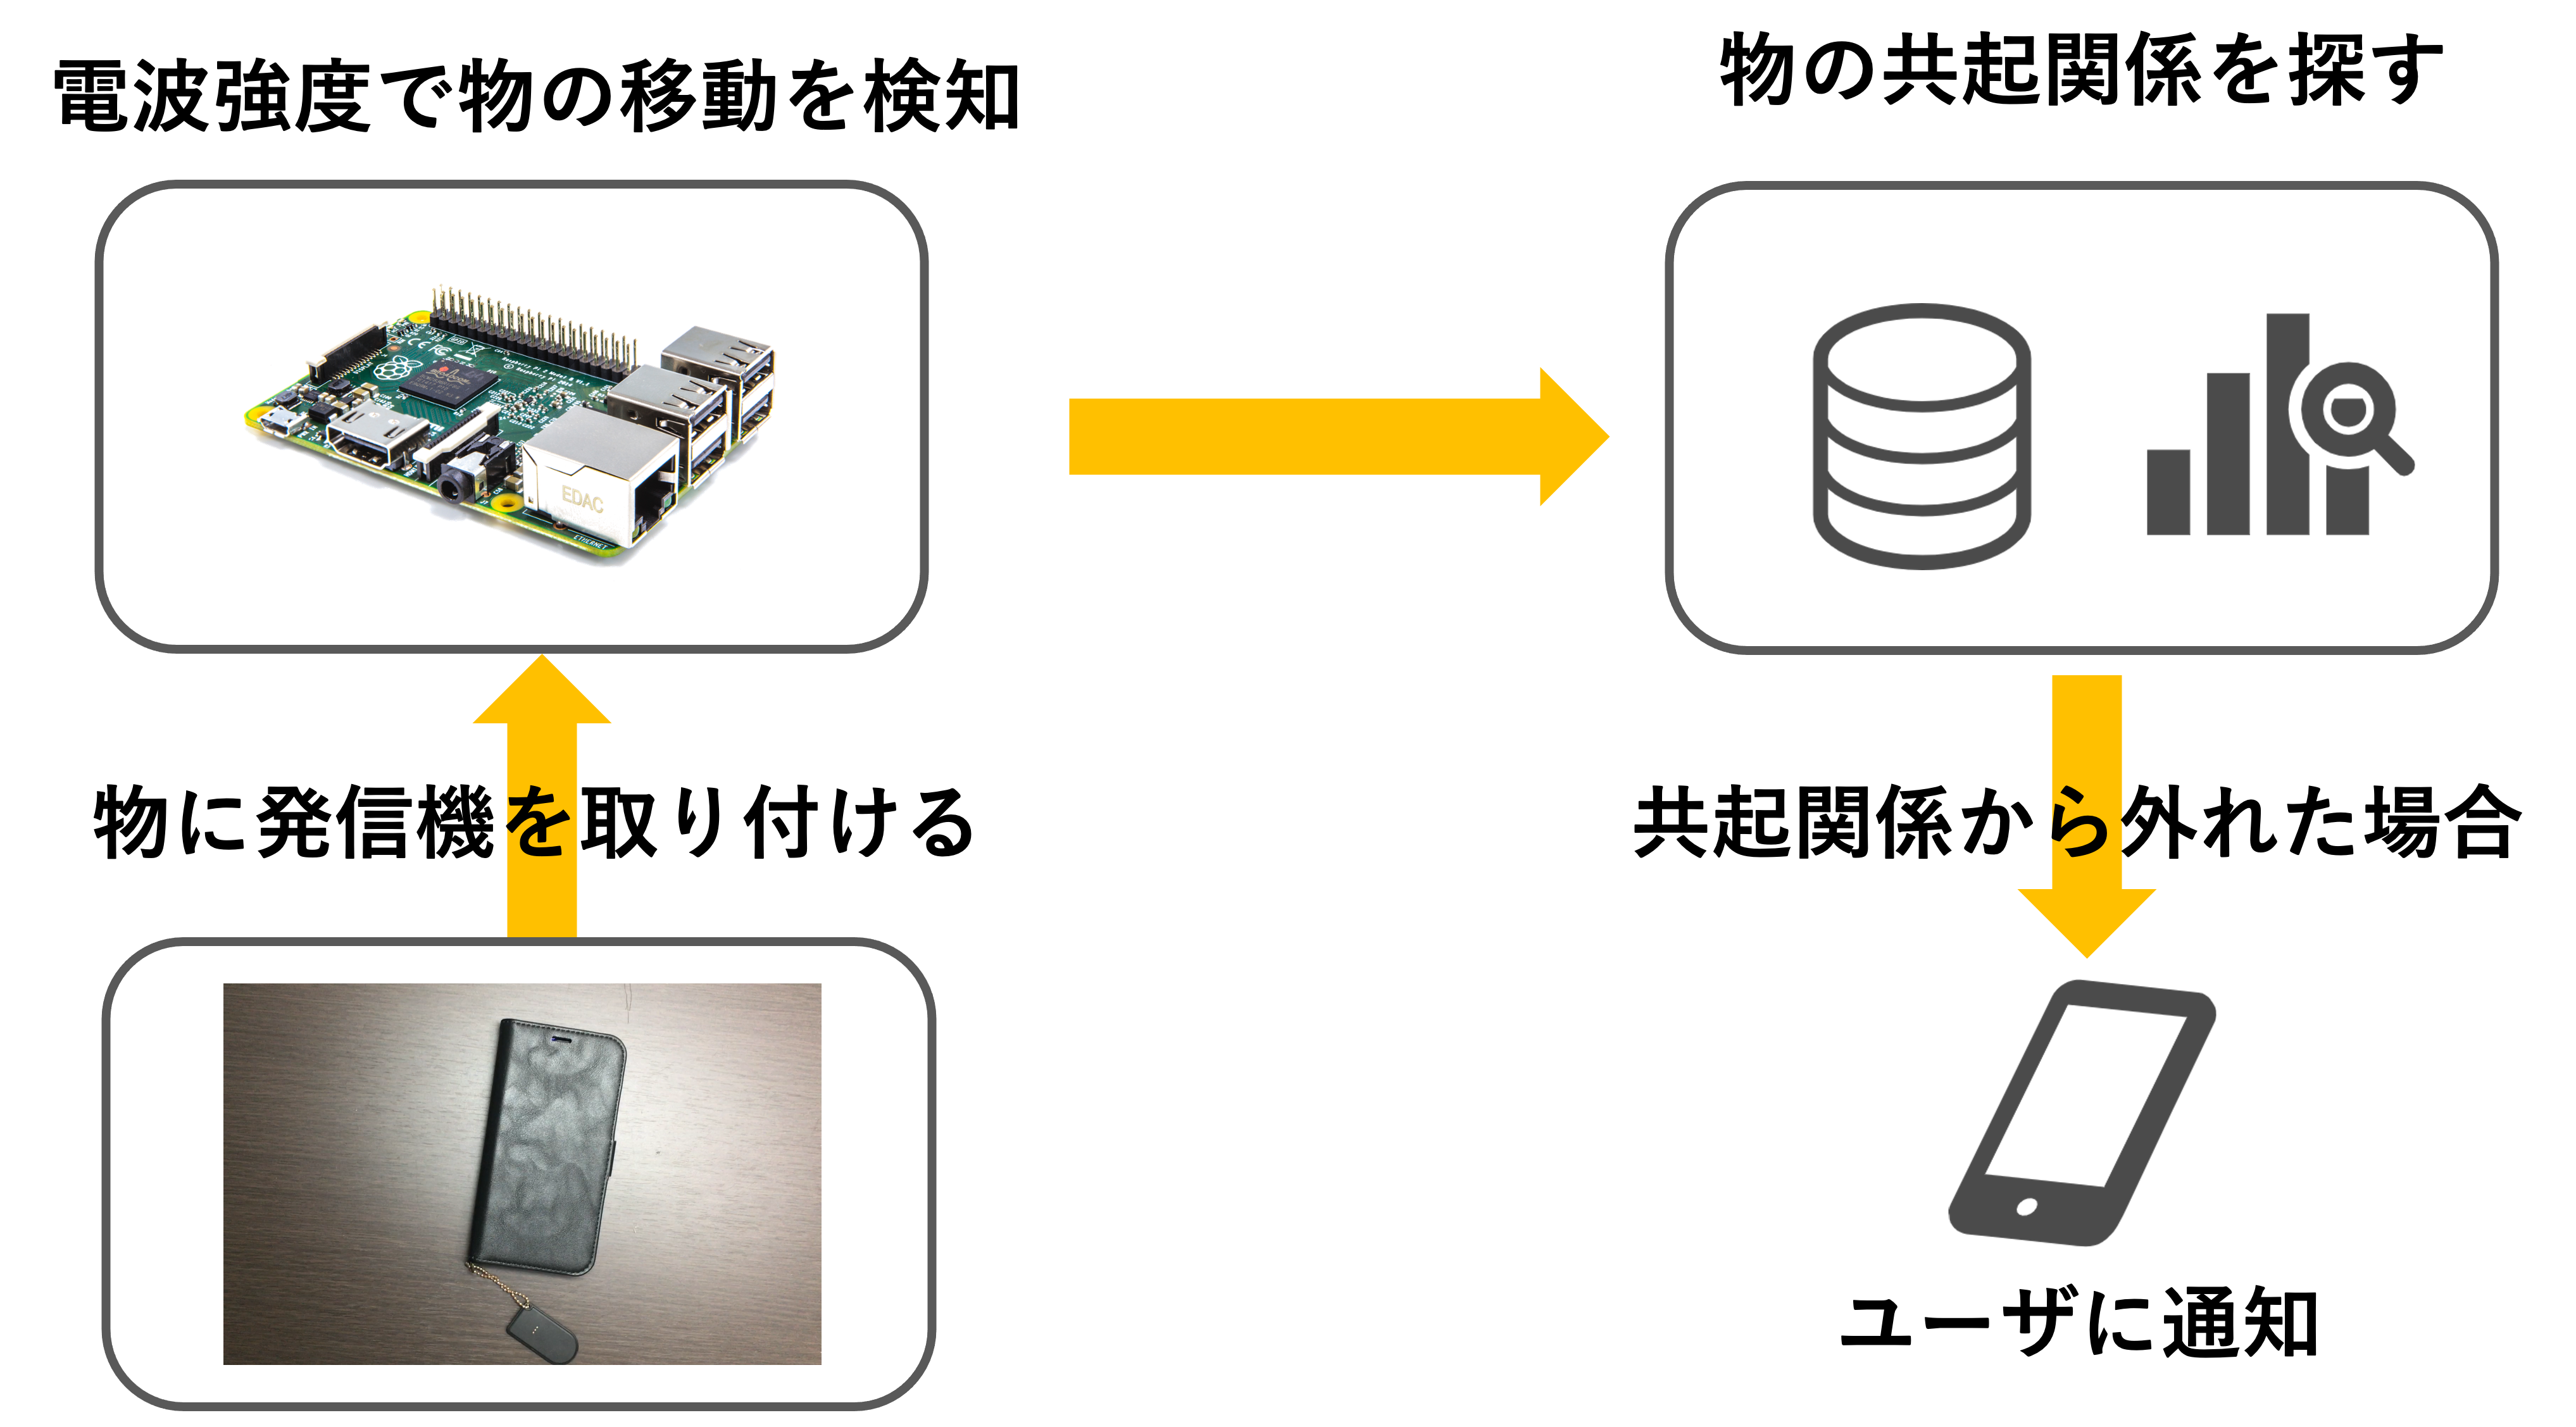
\includegraphics[ width = 80mm]
         {p3.png}
    \caption{システム構成図}
\end{figure}

\subsection{物の場所推定}

物同士の共起関係を調べるには物がどこにあるかを推定し,どこからどこへ移動したかを推定する必要がある.
物の場所を推定する手法として一般的に発信機の電波強度を受信機で受け取る手法がある.
本システムでは特定の場所から特定の場所へ移動する際のそれぞれの場所に受信機を設置する.
例としてリビングから玄関への移動の様子を捉えたい場合は図2,図3のようにリビングと玄関のそれぞれに受信機を設置する.

\begin{figure}[tbh]
    \centering
    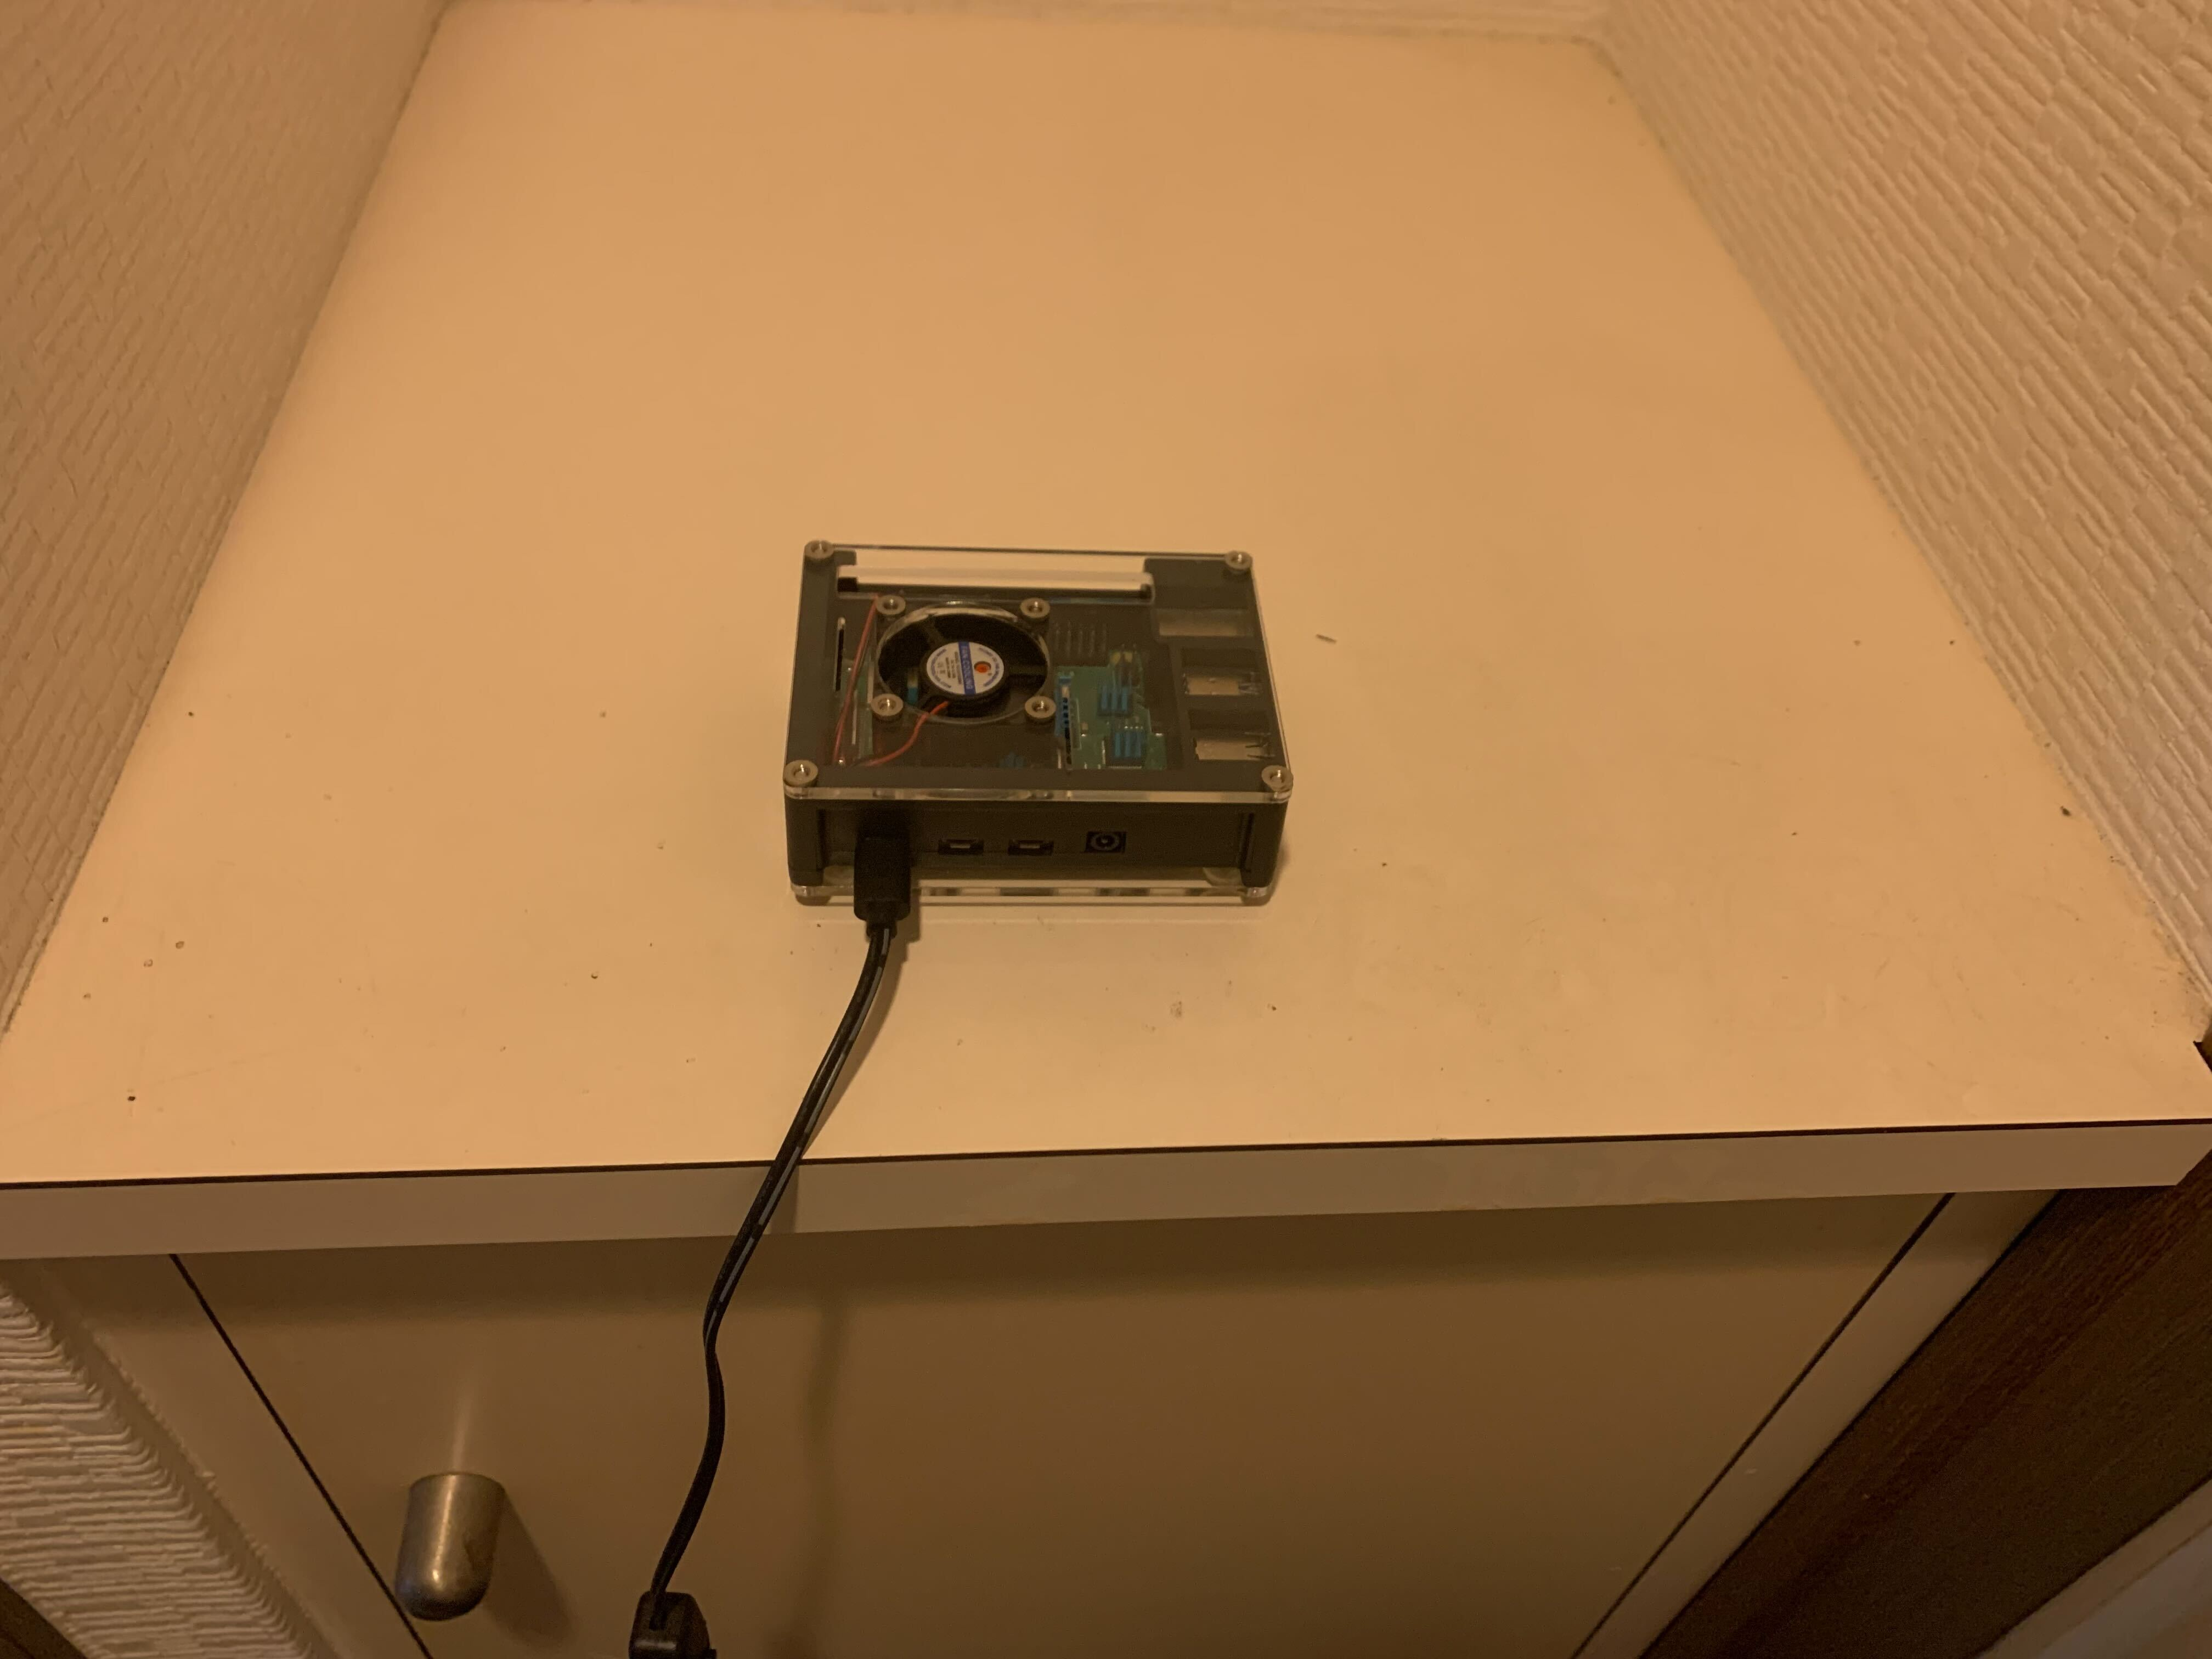
\includegraphics[ width = 70mm]
         {p1.jpg}
    \caption{玄関に設置した受信機}
\end{figure}

\begin{figure}[tbh]
    \centering
    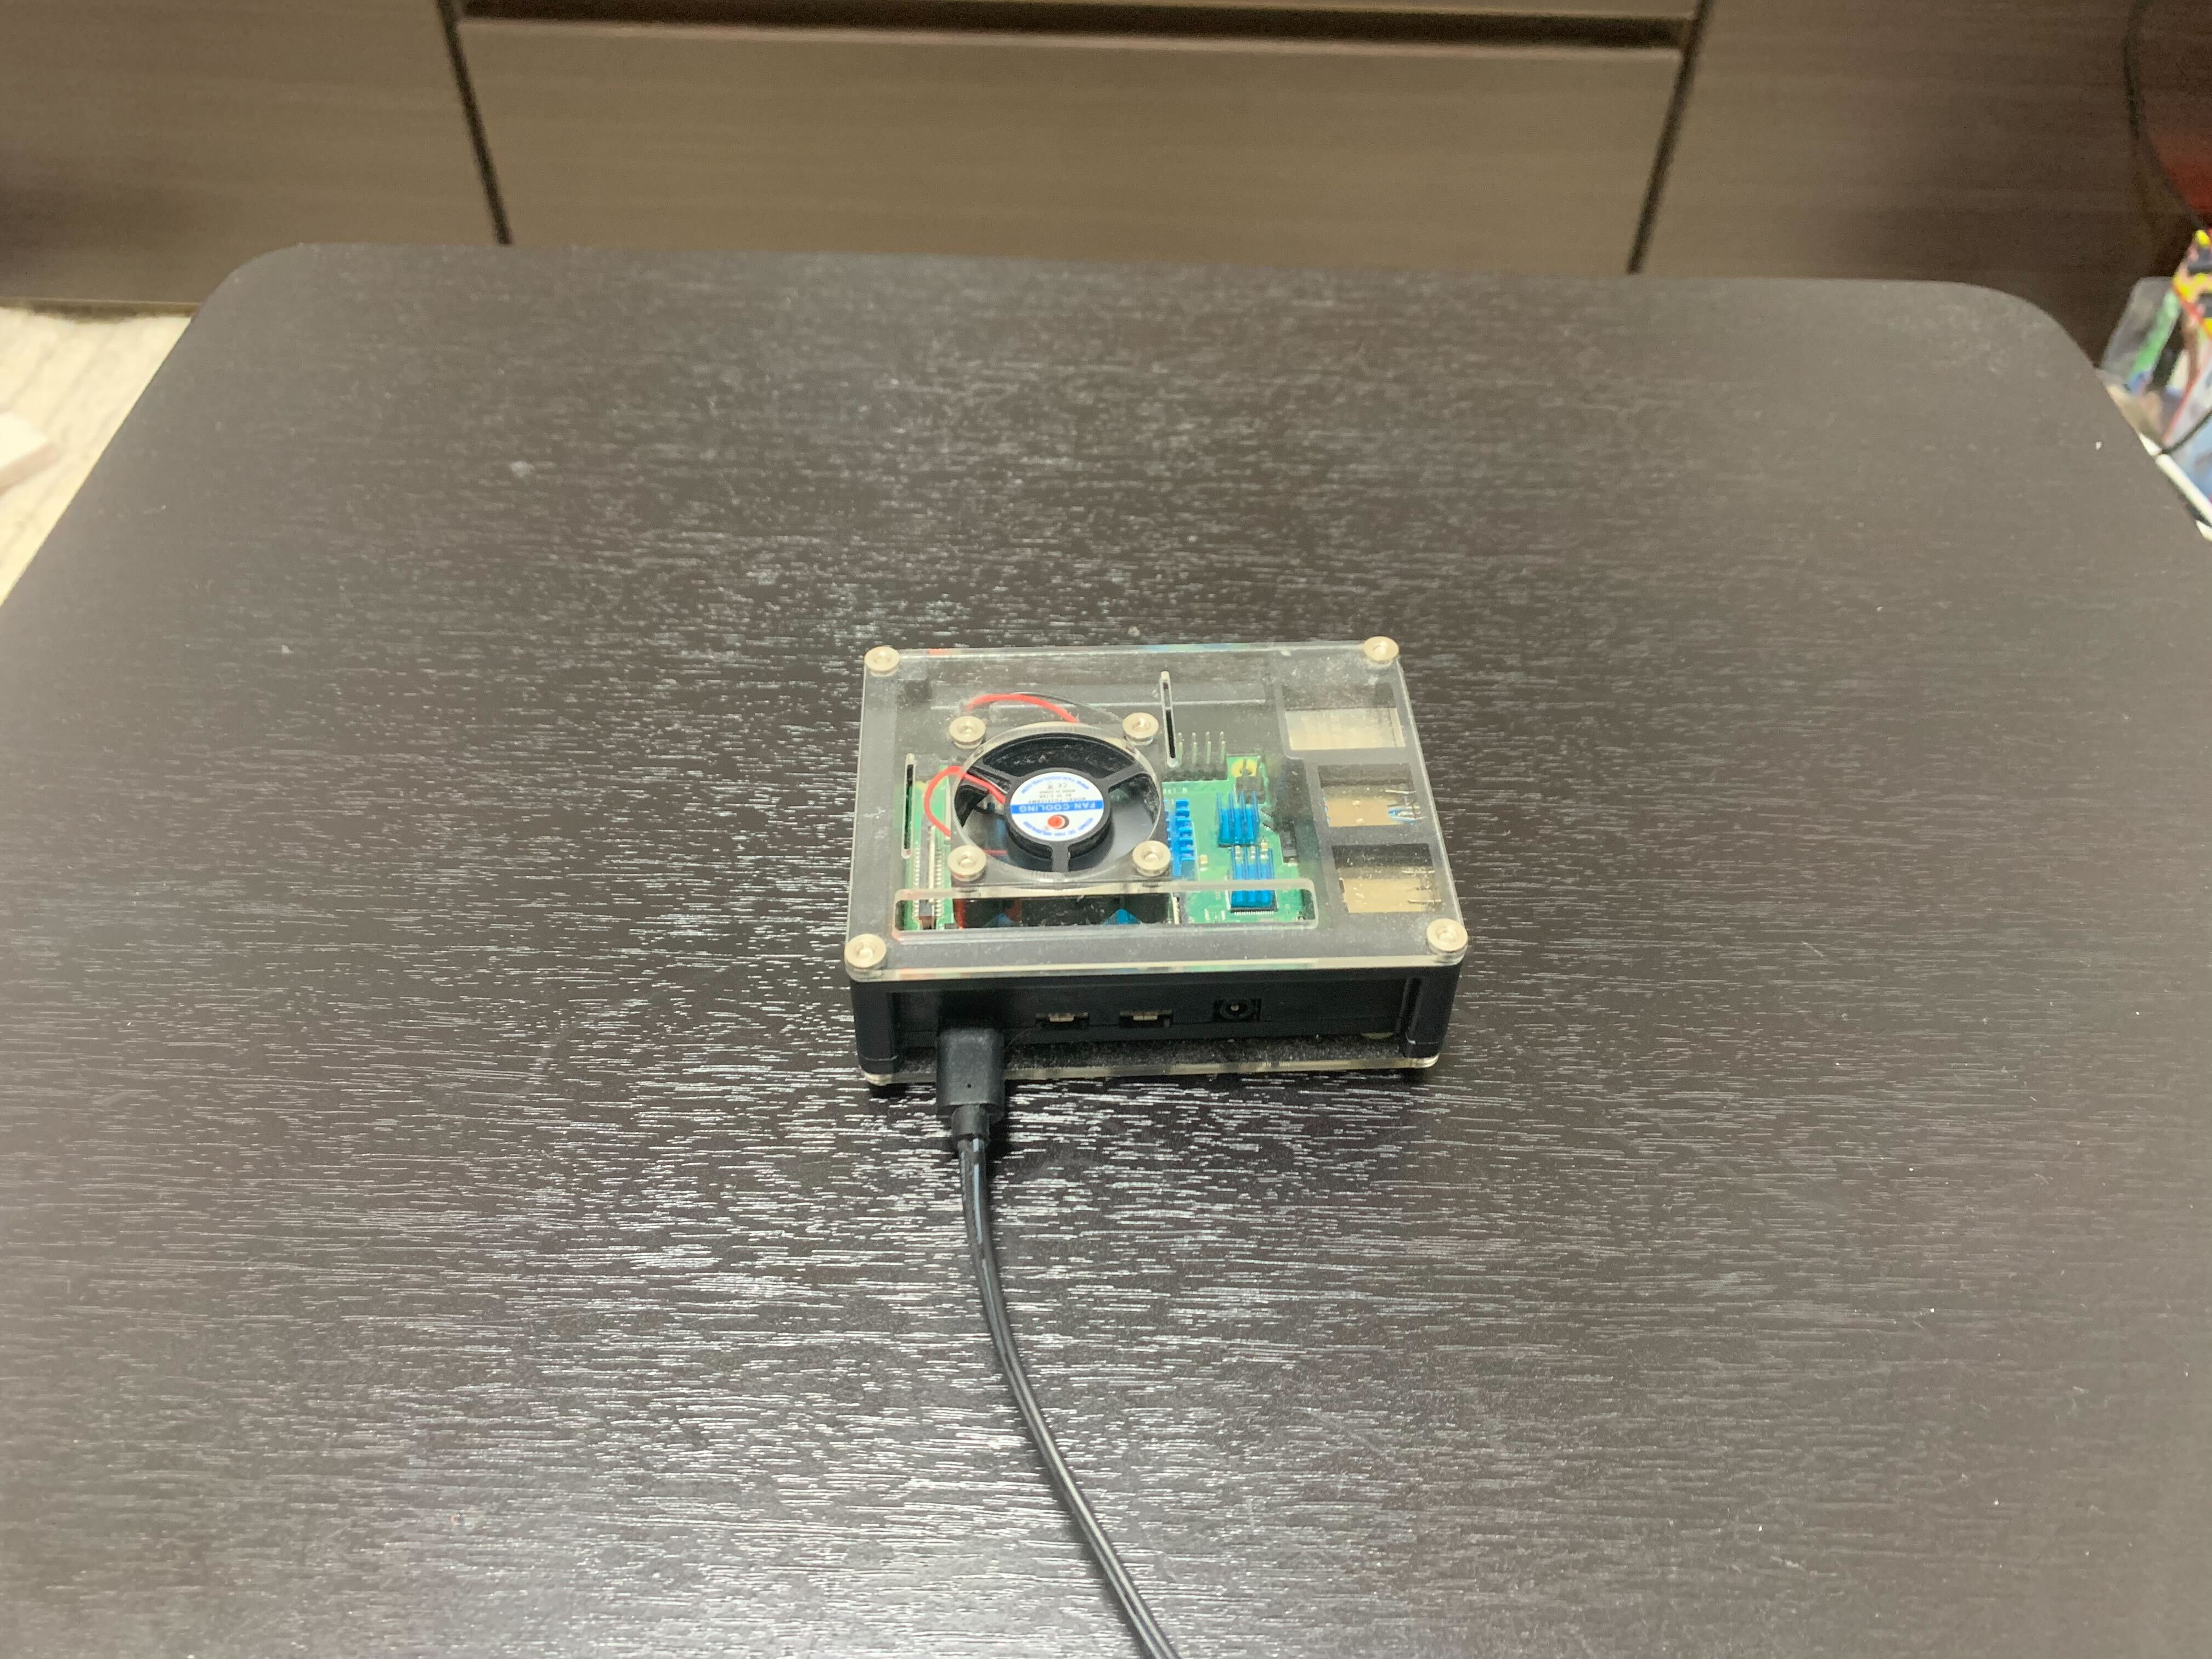
\includegraphics[ width = 60mm]
         {p2.jpg}
    \caption{リビングに設置した受信機}
\end{figure}

物の場所を推定するために置き忘れを検知したい物に発信機を取り付ける.
スマートフォンに発信機を取り付けた例を以下の図4に示す.

\begin{figure}[tbh]
    \centering
    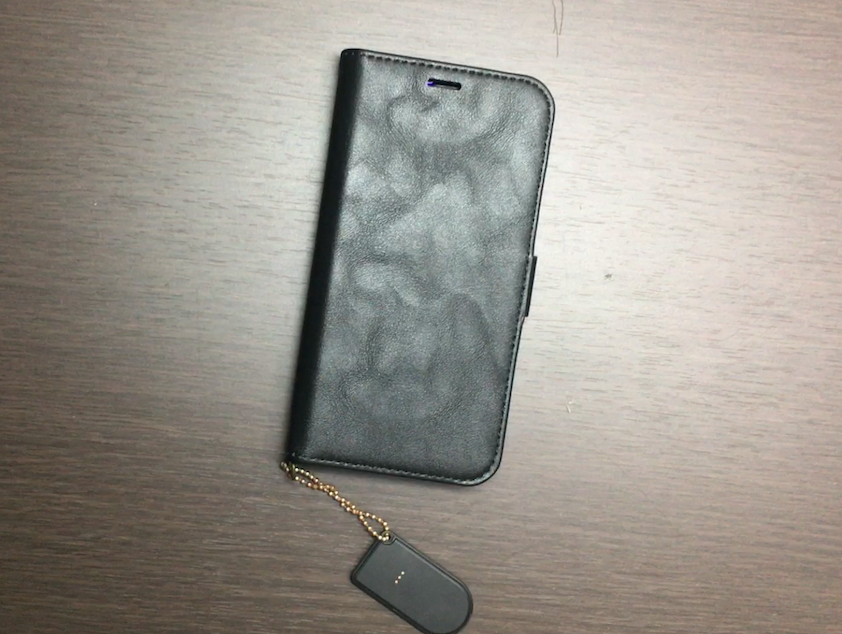
\includegraphics[ width = 60mm]
         {phone3.png}
    \caption{発信機を取り付けた物の例}
\end{figure}

発信器から定期的に送信される情報を2つの受信機で同時に受信し電波強度の比較を行う.
電波強度を比較しより電波強度が強い方に発信機があるという推定結果を出し,
どちらの受信機でも電波が受信できなかった場合,発信機が圏外(家の外)にあると判定結果を出す.
圏外の判定がしばらく続いた場合は外出中の判定をし,この結果は持ち物の推定に用いる.

どの場所にあるかの情報をもとに場所の移動指定を行い,
どの場所にいるかの推定結果が変わった場合に場所の移動が行われた判定を行う.



\subsection{物の共起関係の探索}

物が時空間的な共起関係にあるかを推定するためにはクラスタリングを行い,時間的な類似関係を持つデータをグループ化する必要がある.

クラスタリングの手法としてk-means法や群平均法やウォード法がある.
本システムでは多数のデータから時間的な共起関係を推定するために,最適なクラスタ数を自動で求める手法であるX-means法を採用した.
クラスタリングの例として以下の図5を示す.
図5は8時に朝から学校へ行くためにスマホと財布を持って外出,
12時に昼から学校へ行くためにスマホと財布を持って外出,
16時に買い物へ行くため財布を持って外出,
21時にバイトに行くため財布と通勤用カバンを持って外出,
の4種類の外出しかしない場合のヒストグラムである.
\begin{figure}[tbh]
    \centering
    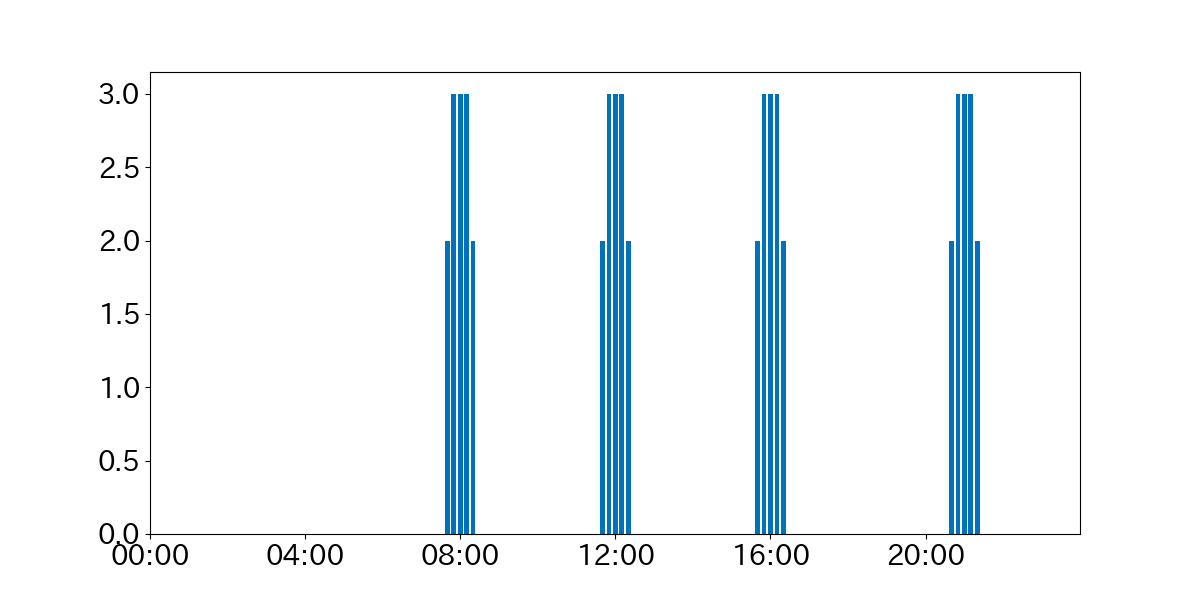
\includegraphics[ width = 80mm]
         {Figure_3.png}
    \caption{共起関係の例}
\end{figure}

図5の例をX-means法を用いてクラスタリングしてクラスタごとに色分けした結果が以下の図6である.

\begin{figure}[tbh]
    \centering
    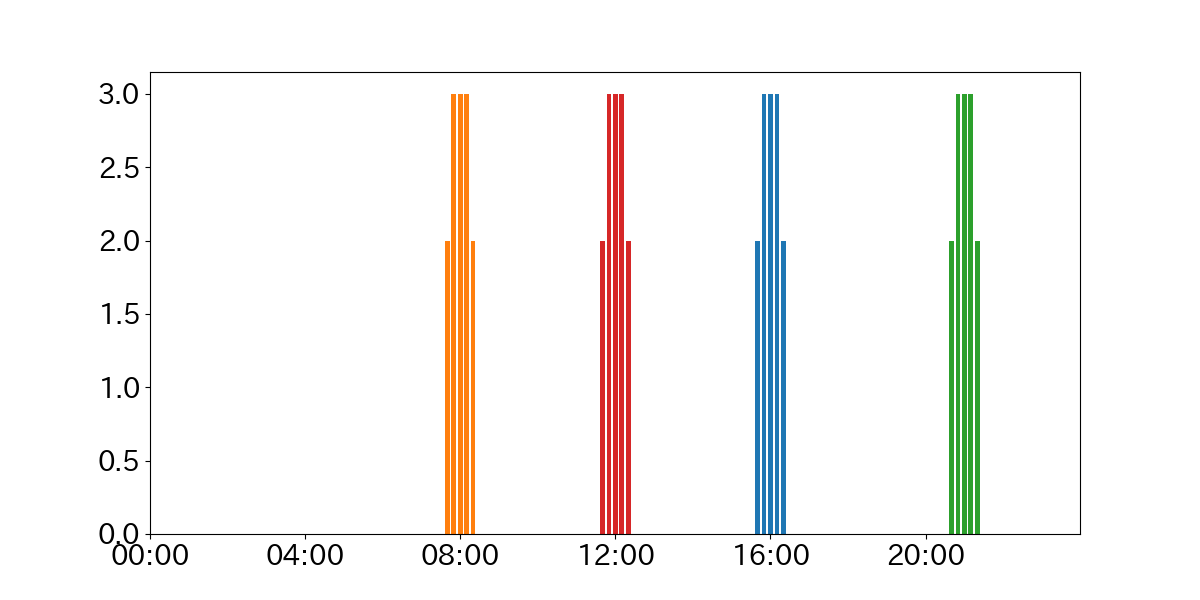
\includegraphics[ width = 80mm]
         {Figure_4.png}
    \caption{共起関係の例をクラスタリングした結果}
\end{figure}

このようにクラスタリングによるグループ化をした後に外出時刻とその際の持ち物から時空間的な共起関係にあるかの推定を行う.


\subsection{データ分析}

各クラスタごとに持ち物の傾向を物同士の組み合わせによる共起関係を用いてデータ分析を行う.
データ分析は外出時刻と持ち物のデータを用いて行い,クラスタごとの平均外出時刻,標準偏差,それらを用いた信頼区間,
各持ち物の組み合わせを持っている確率を求める.
平均値と標準偏差の差の絶対値をσとしてある時間データが与えられた時に,各クラスタの平均値からσの何倍離れているかを計算し,
その値が最小のクラスタに所属していると推定する.

持ち物の組み合わせを予想する手法として事前に手入力で決めたり,ユーザがフィードバックしたりする方法があるが,
本研究では外出に限らず特定の駆動をするときの物の共起関係を求めるので,
クラスタ内における外出の回数の中で何回持ち物の組み合わせを持っていたか,の割合で持っている確率を予想する手法を採用した.



\subsection{ユーザに知らせる}

分析したデータをもとに予想される行動とは違った行動がされた場合,つまり今回の場合は置き忘れがあった場合にユーザに知らせるために,
本システムでは連絡用ツールで通知するシステムを実装する.

移動する直前にユーザに知らせるには物の場所をリアルタイムに取得する必要があり,
移動する直前と判断した場合はその際の持ち物と時間情報を取得し,どのクラスタを参照するかを決定する.
どのクラスタを参照するか決定した後に現在持っている物と,その時間帯の移動の際に持っていると予想される持ち物を比較し,
実際の持ち物と予想された持ち物が違う場合には置き忘れがあると推定しユーザへ知らせる.

ユーザへ置き忘れを知らせる方法として連絡用ツールの中からSlackを採用した.
研究室内での連絡用ツールとして普段から使用しているためである.
通知の手法としてSlackのチャンネルのURLを取得し,そのURLに対してbotでメッセージを送信する方法をとっている.

% ------------------------------------------------------------
\section{評価}

\subsection{外出検知}

本研究では受信機としてRasberry Piを採用し発信器としてBLEビーコンを採用した.
BLEビーコンは小型の機器で物に取り付けやすく,一度電池を交換すると最長1年と似た機能を持った機器と比べて
電池持ちがよいためユーザ側の保守作業の手間が省けると判断した.

本実験環境下では玄関にいると推定された後15秒以上リビング以外の場所にいる状態が続くと「外出直前」という判定を出す.
これの秒数は家の構造にもよるが,リビングを出て靴を履きドアを開けて外出するまでに十分な時間と判断しこの値を設定した.
推定された場所と時間情報をもとに部屋の移動の様子を推定し各発信機に対し「何時から何時までどこにいたか」というデータを生成する.
そのデータをもとに外出時刻が近似している発信機があればそれらを一緒に持って外出したと推定し,外出履歴として外出時刻と持ち物を
データベースに保存する.

この手法は物の移動をある程度正確に検知できるが,
外出の際に持ち物を1つ以上持った状態で玄関に一定時間いると,その時点で外出直前と誤判定されてしまったり,
ビーコンを取り付ける物の状態によっては電波が妨害され正しく動かなくなったりする問題点がある.


\subsection{クラスタリング}

外出時刻と外出回数に着目するといくつかの山が確認できる.以下の図5は自身の平日に限った外出履歴をヒストグラム化した物である.

\begin{figure}[tbh]
    \centering
    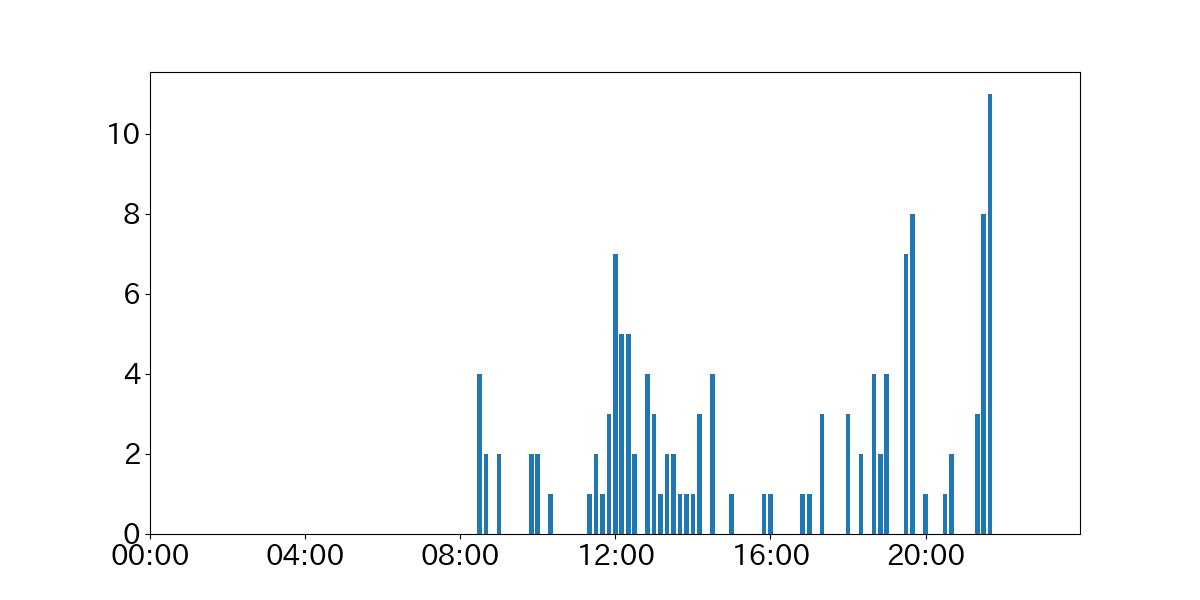
\includegraphics[ width = 80mm]
         {Figure_1.png}
    \caption{平日の外出の様子}
\end{figure}

典型的な例として8時付近は朝から学校に行く時に通学用カバンとスマホと財布と鍵を持って外出し,12時付近は昼から学校に行く時に通学用カバンとスマホと財布と鍵を持って外出し,
16時付近は買い物に行ったり遊びに行ったりする時にスマホと財布とカバンを持って外出し,20時付近はアルバイトに行く時に通勤用カバンとスマホを持って外出をする例があるとする.

本システムでは時間毎の外出傾向を分析するために,データ間の類似度にもとづいてデータをグループ分けするクラスタリングを行い,
クラスタリングの手法の中からX-means法を採用した.この手法は最適なクラスタ数を自動で求める物であるため,
時間ごとの行動分析をするには最適だと判断したためである.

図5のヒストグラムをX-means法でクラスタリングした物を以下の図6に示す.

\begin{figure}[tbh]
    \centering
    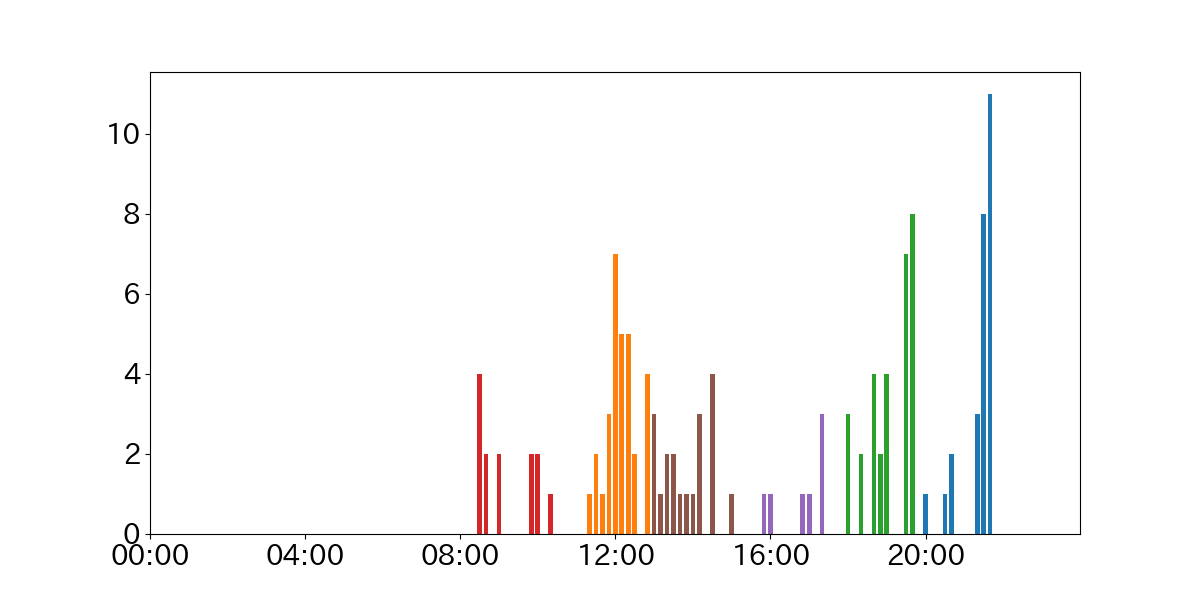
\includegraphics[ width = 80mm]
         {Figure_2.png}
    \caption{クラスタリングの結果}
\end{figure}

8時付近の外出,12時付近の外出,16時付近の外出,20時付近の外出をさらに細かくなっている部分もあるが
ある程度正確にクラスタリングできていることがわかる.

この手法は特定の時間に特定の行動をすることを前提としているので,
例えばバイトに行くために通勤用カバンとスマホを持って外出する場合と,
遊びに行くためスマホと財布を持って外出する場合があるように,
同じような時間に違う特徴を持った外出をする行動をすると持ち物推定の精度が下がってしまう欠点がある.


\subsection{様々な状況下でのデータ分析}
時空間的な物の共起関係を探すためには物の移動と移動の際に一緒に持っている物の2つの情報が必要である.
本システム受信機をリビングと玄関の2箇所に設置し外出の様子に着目したが,
外出以外の移動は,受信機を設置できる環境さえあればある場所から別の場所への移動を捉えられるため対応可能である.
また外出の際に持ち物を捉えるため発信機をスマホ,財布,通勤カバンに取り付けたが,
発信機を取り付ける物が増えた場合でも持ち物の組み合わせのパターンが増えるだけなのでこちらも対応可能である.


\subsection{ユーザへの通知方法}
ユーザへ置き忘れを知らせる方法として,アプリを使って通知する以外に玄関にディスプレイを設置しそこに置き忘れがあれば表示する方法があった.
本システムでは外出しそうという判定をするために15秒以上玄関にいた場合と定義している.
そのため仮に置き忘れをした状態で急いで家を出てしまった場合ディスプレイに置き忘れが表示される前に外出してしまう事になり,
ユーザが置き忘れに気づくのは置き忘れた物が必要になった時で手遅れになってしまう.

一方スマホに通知する場合は通知音やバイブレーションを伴うので,
仮に急いで家を出た場合でも通知にさえ気づけば置き忘れを防止できる.

しかし本システムは外出時にスマホをほぼ必ず持っているという前提条件が存在してしまうため,
普段からスマホをあまり持ち歩かない人や基本的にスマホを見ない人に対しては効果が失われてしまう欠点がある.

\section{おわりに}
\subsection{まとめ}

本研究では物の時空間的な共起関係に基づいた行動パターンを生成し,分析を行い実際の結果と比較することでユーザに置き忘れを通知する
システムの開発を行った.

各場所に受信機を,置き忘れを検知したい物には発信機を取り付け電波強度の比較を行い物の移動を推定する.
物が移動した際に一緒に移動していた物は時空間的な共起関係にあると判断して外出時刻と持ち物のデータを集める.
クラスタリングを行い外出した時にどの持ち物を持っていそうか判定を行う.
持っていそうな物を実際に持っていない場合は通知を行う.


\subsection{今後の課題}
今後の課題として同じような時間に別の行動をした際の区別をする手法の探索や
そもそもスマホをあまり見ない人に対してどのように置き忘れを気づかせるか,
が挙げられる.

外出の際の持ち物と移動先を紐づけた情報を与えることで,同じような時間の別の行動でも区別できるので
データ分析の際に必要なデータを見直し持ち物推定の精度を上げる必要がある.



% ------------------------------------------------------------
\begin{thebibliography}{9}


\bibitem{1}
田中未来哉, 角所考,小島隆次. 人物行動を手掛かりとした放置物体の置き忘れ検出可能性の検討.
ヒューマンインタフェース学会論文誌 23.2 (2021): 209-212.

\bibitem{2}
青田慎也, 吉田博哉, RFID による忘れ物防止システムの実現性の考察.
第 76 回全国大会講演論文集 2014.1 (2014): 397-398.

\bibitem{3}
北園優希, 井上剛志, 宮内真人, 芹川聖一. (2008). 加速度センサと RFID タグを用いた置き忘れ防止システムの開発. 
電気学会論文誌 E (センサ・マイクロマシン部門誌), 128(9), 364-365.

\bibitem{4}
山岡澪奈, 飯島安恵, 今野将. 忘れ物防止支援システムのための所持傾向の分析. 
第 16 回情報科学技術フォーラム (FIT2017) 講演論文集, 2017, 16.2: 141-142.

\bibitem{5}
浜野悠介, 高橋伸, 田中二郎. (2013). 持ち物の組み合わせを重さから推定するシステム. 
第 75 回全国大会講演論文集, 2013(1), 89-90.

\bibitem{6}
森田陽介, 内田真人, 山岡澪奈, 飯島安恵, 今野将. (2018). 持ち物推薦システムのための所持履歴取得機能の開発. 
第 80 回全国大会講演論文集, 2018(1), 357-358.

\bibitem{7}
中田豊久, et al. スポットライトによる物探し支援システム. 
情報処理学会研究報告グループウェアとネットワークサービス (GN), 2005, 2005.30 (2004-GN-055): 25-30.


\bibitem{8}
佐藤喬, et al. 低価格カメラを使った探し物支援システム. 
全国大会講演論文集, 2009, 人工知能と認知科学: 11-12.


\bibitem{9}
上岡隆宏, et al. I’m here!: 物探しを効率化するウェアラブルシステム. 
ヒューマンインタフェース学会論文誌, 2004, 6.3: 275-285.















\end{thebibliography}


% ------------------------------------------------------------
\end{document}
